\documentclass[tikz,border=4pt]{standalone}
\usepackage{amsmath,amssymb}\renewcommand{\familydefault}{\sfdefault}
\usepackage{pgfplots}\pgfplotsset{compat=1.17}
\usetikzlibrary{arrows.meta,positioning,shadows,fit,calc,backgrounds,patterns}
\definecolor{lav}{HTML}{E6E6FF}\definecolor{pinkb}{HTML}{FFDDDD}\definecolor{greenb}{HTML}{DDFFDD}\definecolor{yelb}{HTML}{FFFBCF}\definecolor{peach}{HTML}{FFEBD6}\definecolor{mauve}{HTML}{F0E6F0}
\definecolor{reqblue}{HTML}{0000BB}\definecolor{resgreen}{HTML}{008800}\definecolor{dred}{HTML}{CC0000}\definecolor{domblue}{HTML}{000099}\definecolor{crimson}{HTML}{990033}
\definecolor{tbBlue}{HTML}{1F77B4}\definecolor{tbOrange}{HTML}{FF7F0E}\definecolor{tbGreen}{HTML}{2CA02C}\definecolor{tbRed}{HTML}{D62728}\definecolor{tbPurple}{HTML}{9467BD}\definecolor{tbBrown}{HTML}{8C564B}
\definecolor{barGreen}{HTML}{1B8754}\definecolor{darkGreen}{HTML}{2E7D32}\definecolor{lightBlue}{HTML}{A0C4FF}\definecolor{kRed}{HTML}{DC3545}
\definecolor{accB}{HTML}{3366FF}\definecolor{f1O}{HTML}{FF7F50}\definecolor{aucG}{HTML}{44CC11}
\tikzset{node/.style={draw,rounded corners=2.5pt,thick,align=center},
 req/.style={-{Stealth[length=2.4mm]},thick,reqblue},res/.style={-{Stealth[length=2.4mm]},thick,dashed,resgreen}}
\pgfplotsset{every axis/.append style={tick label style={font=\footnotesize},label style={font=\small},title style={font=\small},legend style={font=\footnotesize,fill=white,fill opacity=.9,text opacity=1,draw=black!25,rounded corners=1pt},
 grid style={dotted,black!35}}}
\begin{document}
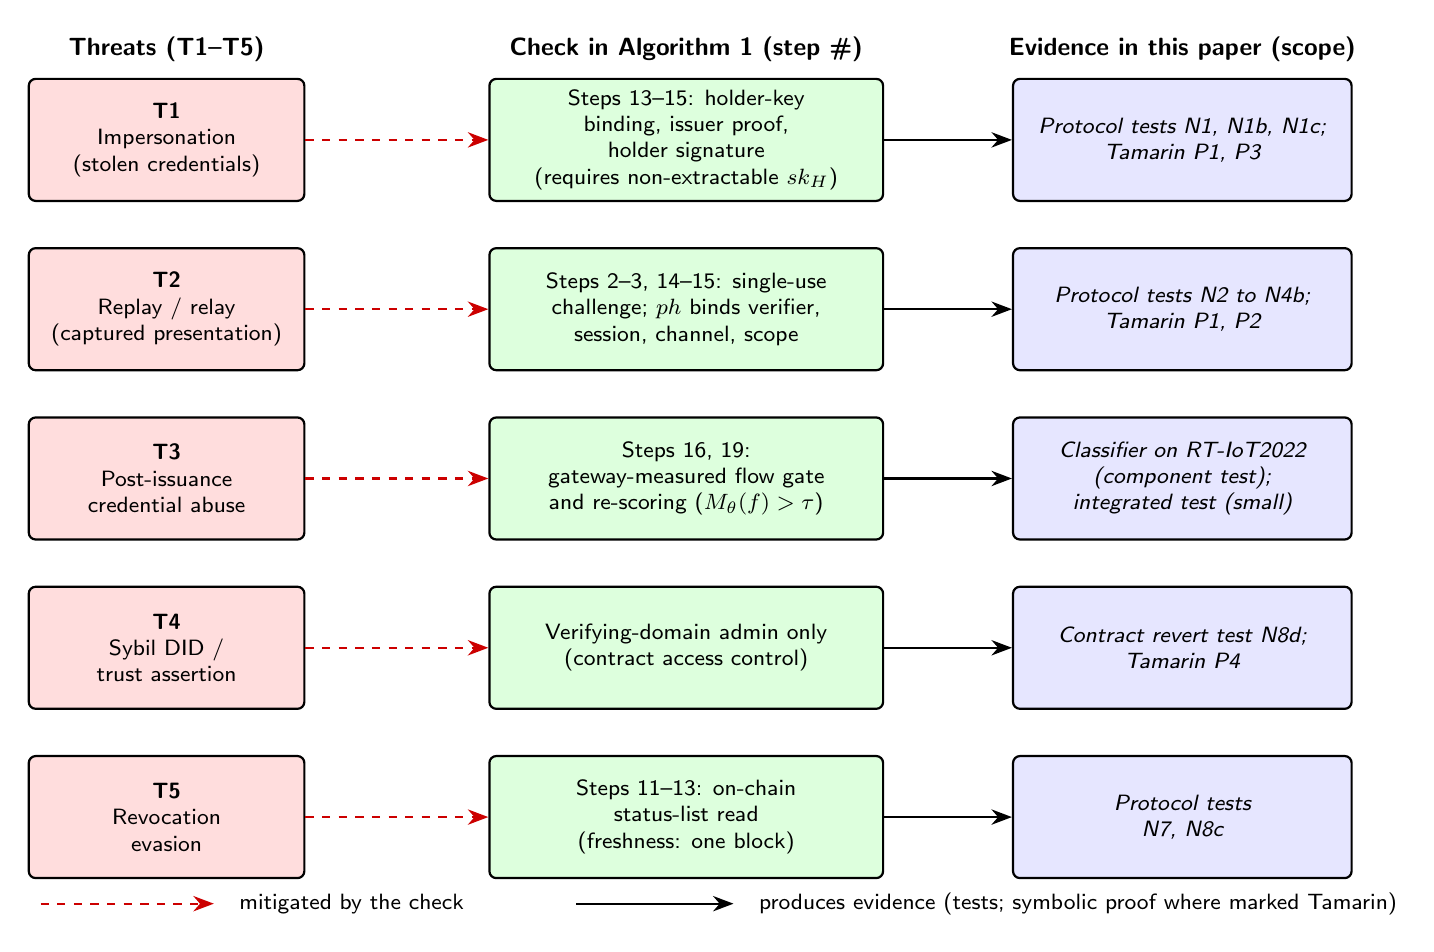
\begin{tikzpicture}[font=\small]
\node[font=\bfseries\small] at (0,1.15) {Threats (T1--T5)}; \node[font=\bfseries\small] at (6.6,1.15) {Check in Algorithm 1 (step \#)}; \node[font=\bfseries\small] at (12.9,1.15) {Evidence in this paper (scope)};
\node[node,fill=pinkb,minimum width=3.5cm,minimum height=1.55cm,font=\footnotesize] (t0) at (0,0.0) {\textbf{T1}\\Impersonation\\(stolen credentials)};
\node[node,fill=greenb,minimum width=5.0cm,minimum height=1.55cm,font=\footnotesize] (c0) at (6.6,0.0) {Steps 13--15: holder-key\\binding, issuer proof,\\holder signature\\(requires non-extractable $sk_H$)};
\node[node,fill=lav,minimum width=4.3cm,minimum height=1.55cm,font=\footnotesize\itshape] (e0) at (12.9,0.0) {Protocol tests N1, N1b, N1c;\\Tamarin P1, P3};
\draw[-{Stealth[length=2.6mm]},thick,dashed,dred] (t0) -- (c0); \draw[-{Stealth[length=2.6mm]},thick] (c0) -- (e0);
\node[node,fill=pinkb,minimum width=3.5cm,minimum height=1.55cm,font=\footnotesize] (t1) at (0,-2.15) {\textbf{T2}\\Replay / relay\\(captured presentation)};
\node[node,fill=greenb,minimum width=5.0cm,minimum height=1.55cm,font=\footnotesize] (c1) at (6.6,-2.15) {Steps 2--3, 14--15: single-use\\challenge; $ph$ binds verifier,\\session, channel, scope};
\node[node,fill=lav,minimum width=4.3cm,minimum height=1.55cm,font=\footnotesize\itshape] (e1) at (12.9,-2.15) {Protocol tests N2 to N4b;\\Tamarin P1, P2};
\draw[-{Stealth[length=2.6mm]},thick,dashed,dred] (t1) -- (c1); \draw[-{Stealth[length=2.6mm]},thick] (c1) -- (e1);
\node[node,fill=pinkb,minimum width=3.5cm,minimum height=1.55cm,font=\footnotesize] (t2) at (0,-4.3) {\textbf{T3}\\Post-issuance\\credential abuse};
\node[node,fill=greenb,minimum width=5.0cm,minimum height=1.55cm,font=\footnotesize] (c2) at (6.6,-4.3) {Steps 16, 19:\\gateway-measured flow gate\\and re-scoring ($M_\theta(f)>\tau$)};
\node[node,fill=lav,minimum width=4.3cm,minimum height=1.55cm,font=\footnotesize\itshape] (e2) at (12.9,-4.3) {Classifier on RT-IoT2022\\(component test);\\integrated test (small)};
\draw[-{Stealth[length=2.6mm]},thick,dashed,dred] (t2) -- (c2); \draw[-{Stealth[length=2.6mm]},thick] (c2) -- (e2);
\node[node,fill=pinkb,minimum width=3.5cm,minimum height=1.55cm,font=\footnotesize] (t3) at (0,-6.449999999999999) {\textbf{T4}\\Sybil DID /\\trust assertion};
\node[node,fill=greenb,minimum width=5.0cm,minimum height=1.55cm,font=\footnotesize] (c3) at (6.6,-6.449999999999999) {Verifying-domain admin only\\(contract access control)};
\node[node,fill=lav,minimum width=4.3cm,minimum height=1.55cm,font=\footnotesize\itshape] (e3) at (12.9,-6.449999999999999) {Contract revert test N8d;\\Tamarin P4};
\draw[-{Stealth[length=2.6mm]},thick,dashed,dred] (t3) -- (c3); \draw[-{Stealth[length=2.6mm]},thick] (c3) -- (e3);
\node[node,fill=pinkb,minimum width=3.5cm,minimum height=1.55cm,font=\footnotesize] (t4) at (0,-8.6) {\textbf{T5}\\Revocation\\evasion};
\node[node,fill=greenb,minimum width=5.0cm,minimum height=1.55cm,font=\footnotesize] (c4) at (6.6,-8.6) {Steps 11--13: on-chain\\status-list read\\(freshness: one block)};
\node[node,fill=lav,minimum width=4.3cm,minimum height=1.55cm,font=\footnotesize\itshape] (e4) at (12.9,-8.6) {Protocol tests\\N7, N8c};
\draw[-{Stealth[length=2.6mm]},thick,dashed,dred] (t4) -- (c4); \draw[-{Stealth[length=2.6mm]},thick] (c4) -- (e4);
\draw[-{Stealth[length=2.6mm]},thick,dashed,dred] (-1.6,-9.7) -- (0.6,-9.7); \node[anchor=west,font=\footnotesize] at (0.8,-9.7) {mitigated by the check};
\draw[-{Stealth[length=2.6mm]},thick] (5.2,-9.7) -- (7.2,-9.7); \node[anchor=west,font=\footnotesize] at (7.4,-9.7) {produces evidence (tests; symbolic proof where marked Tamarin)};
\end{tikzpicture}
\end{document}
